%----------------------------------------------------------------------------
\chapter{Monitor forráskód generálás}\section{Időzített automata generátor}
%----------------------------------------------------------------------------

%----------------------------------------------------------------------------
\subsection{Az automata generátor célja}
%----------------------------------------------------------------------------

Az \textit{Önálló laboratórium} során elkészített automata generátort kibővítettem úgy, hogy támogassa a \textit{TPSC} elemekhez tartozó automata minták generálását.
Az eredeti automata generátor \textit{PSC} szöveges leírásokhoz tartozó \textit{Büchi} automatákat tudta összeállítani.
Az volt a feladatom, hogy a meglévő \textit{Büchi} automata mintákat lecseréljem a korábban ismertetett időzített automata mintákra és felvegyem a hiányzó mintákat, amelyek az időzítési feltételeket tartalmazó üzenetekhez tartoznak.
A kibővített automata generátor bemenetként egy \textit{TPSC} szcenárió szöveges leírását kapja meg, amelyből a minta alapú módszerrel generál egy \textit{TA} automatát.

A \ref{tpsc_alt} és \ref{tpsc_alt_nc} kódrészleteken látható, hogy a monitor generátor támogatja az összetett operátorokat tartalmazó \textit{TPSC}-khez tartozó \textit{TA}-k generálását is.
A generátor készít egy szöveges leírást a generált automatához, ehhez a \textit{Never claim} nyelvet használja.
A \textit{Never claim} \cite{NeverClaim} a \textit{Promela} nyelv része, ezzel egy rendszer viselkedését lehet definiálni.
Egy \textit{Never claim} leírás a \textit{never} kulcsszóval kezdődik és '\{' '\}' jelek között vannak az automata állapotai lista szerűen felsorolva egymás alatt.
Minden állapothoz tartozó kimenő átmenet az \textit{if} és \textit{fi} kulcssavak között található.
Egy átmenet leírása a címkéjét tartalmazza és egy \textit{$\,\to\,$} jelzi, hogy melyik állapotba visz át.
A \ref{tpsc_alt} kódrészleten lévő szöveges \textit{TPSC} leíráshoz tartozó generált automata \textit{Never claim} leírását a \ref{tpsc_alt_nc} kódrészlet tartalmazza.
Továbbá a generátor képes az üzenet paraméterek kezelésére.
%Például az \textit{alt} operátor feltételét képes feldolgozni és azt elhelyezni a generált automata megfelelő élén.

\begin{lstlisting}[language=java,frame=single, float=h!, caption={\textit{Alt} operátort tartalmazó szcenárió.},captionpos=b,label=tpsc_alt]
specification Bank {

	object UserInterface ui;
	object ATM atm;
	object BankDB db;

	bool success = true;

	constraint b {
		message logout() ui->atm;
	}

	scenario transaction {
		message login(success) ui->atm;

		alt (equals(success, true)) {
			message wReq() ui->atm;
			message uDB() atm->db;
		} (equals(success, false)) {
			message loginUnsuccessful() ui->atm;
			message lockMachine() required atm->ui;
		}
	}
}
\end{lstlisting}

\begin{lstlisting}[language=java,frame=single, float=h!, caption={\textit{Alt} operátort tartalmazó szcenárió \textit{never claim} leírása.},captionpos=b,label=tpsc_alt_nc]
bool success = true;

never{ /*transactionMonitor*/
T0_init:
 if
 :: (!(ui.login(success).atm)) -> goto T0_init
 :: (ui.login(success).atm) -> goto T0_q1
 fi;
T0_q1:
 if
 :: (epsilon) -> goto T0_qinit0
 fi;
T0_qinit0:
 if
 :: (epsilon; success == true) -> goto T0_q2
 :: (epsilon; success == false) -> goto T0_q5
 fi;
T0_qfinal1:
 if
 fi;
T0_q2:
 if
 :: (!(ui.wReq().atm)) -> goto T0_q2
 :: (ui.wReq().atm) -> goto T0_q3
 fi;
T0_q3:
 if
 :: (!(atm.uDB().db)) -> goto T0_q3
 :: (atm.uDB().db) -> goto T0_q4
 fi;
T0_q4:
 if
 :: (epsilon) -> goto T0_qfinal1
 fi;
T0_q5:
 if
 :: (!(ui.loginUnsuccessful().atm)) -> goto T0_q5
 :: (ui.loginUnsuccessful().atm) -> goto T0_q6
 fi;
T0_q6:
 if
 :: (!(atm.lockMachine().ui)) -> goto T0_q6
 :: (!(atm.lockMachine().ui)) -> goto accept_q7
 :: (atm.lockMachine().ui) -> goto T0_q8
 fi;
accept_q7:
 if
 fi;
T0_q8:
 if
 :: (epsilon) -> goto T0_qfinal1
 fi;
}
\end{lstlisting}

%----------------------------------------------------------------------------
\subsection{Az automata generátor megvalósítása}
%----------------------------------------------------------------------------
A generátorhoz az \textit{Xtend} technológiát használtam.
Minden egyes \textit{TPSC} üzenethez legenerálja a hozzá tartozó minta automatát, majd elvégzi azok összecsatolását.

Az időzített automaták generálásához egy adatstruktúrát definiáltam, amely a következő \textit{Java} osztályokból és interfészekből áll:
\begin{itemize}
    %\item AltExpressionInterface
    \item \textit{Automaton}, az automata implementációját tartalmazza, eltárolja az állapotokat és az átmeneteket
    %\item BasicTransition
    \item \textit{ClockConstraint}, időzítési feltételek \textit{Java} implementációját tartalmazza
    %\item ClockExpressionInterface
    \item \textit{Constraint}, megkötések implementációját tartalmazza
    %\item EpsilonTransition
    %\item OperatorFunctions
    \item \textit{State}
    \item \textit{StateType}
    \item Transition
    %\item UnwantedConstraint
    %\item WantedConstraint
\end{itemize}

Az automatában lévő állapotok implementációja a \textit{State} osztályban található.
Két attribútuma van:
\begin{itemize}
	\item id(\textit{String}): az állapot címkéje
	\item type(\textit{StateType}): az állapot típusa
\end{itemize}

Az állapot típusának a megadására a \textit{StateType} \textit{enum} osztályt definiáltam.
Az \textit{enum} a következő értékeket veheti fel:
\begin{itemize}
	\item NORMAL, egy sima állapotot jelöl
	\item ACCEPT, elfogadó állapot jelöl (a monitor szempontjából ez egy hibaállapot)
	\item FINAL, a végállapotot jelöli
\end{itemize}

Az átmenetek implementációjáért felelős osztály a \textit{Transition}.
Három tagváltozója van:
\begin{itemize}
	\item id(\textit{String}): az átmenet címkéje
	\item reset(\textit{String}): visszaállítandó óraváltozó neve
	\item sender(\textit{State}): a forrás állapot
	\item receiver(\textit{State}): a cél állapot
	\item constraint(\textit{Constraint}): az átmeneten lévő megkötés
	\item clockConstraint(\textit{ClockConstraint}): az átmeneten lévő időzítési feltétel
\end{itemize}

Az időzített automata implementációja az \textit{Automaton} osztályban található.
Itt tároljuk az automatában lévő állapotokat és a köztük lévő átmeneteket egy-egy listában.
Az \textit{Automaton} osztály \textit{addState(State)} és \textit{addTransition(Transition)} függvényeivel lehet új állapotot és átmenetet hozzáadni az automatához, a \textit{collapse(Automaton)} függvényével pedig két automatát egyesíteni.
Ezt a függvényt használtam az implementációban a minta automaták egyesítésére, ezen kívül az osztálynak van egy \textit{merge(ArrayList<Automaton>)} függvénye.
Ez a függvény az \textit{alt} operátor ágaiban lévő minta automaták összefésülésére szolgál.

A \textit{Specification} osztály feladata, hogy összeállítsa a szöveges leírásban specifikált \textit{TPSC} szcenárióhoz tartozó időzített automatát.
Ezt követően az automata \textit{Never Claim} leírását egy \textit{.txt} kiterjesztésű fájlba írja.

%----------------------------------------------------------------------------
\subsection{Mintapélda}
%----------------------------------------------------------------------------

\begin{lstlisting}[language=java,frame=single, float=h!, caption={\textit{TPSC} szcenárió szöveges leírása.},captionpos=b,label=tpsc_example_text]
specification Bank {

	object User_Interface ui;
	object ATM atm;
	object BankDB db;

	clock x;

	constraint b {
		message logout() ui -> atm;
	}

	scenario transaction {
		message login() ui -> atm reset x;
		required pastConstraint {b, <(x, 1)} message wReq() ui -> atm clockConstraint {<(x, 5)};
		message uDB() atm -> db clockConstraint {<(x, 10)};
	}
}
\end{lstlisting}

\begin{figure}[h!]
    \centering
    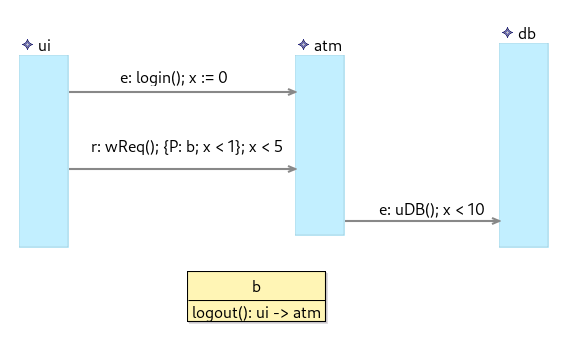
\includegraphics[width=130mm, keepaspectratio]{figures/tpsc_automaton_generator_sirius.png}
    \caption{A \ref{tpsc_example_text} kódrészlet \textit{TPSC} szcenáriójának diagramja.}
	\label{tpsc_example_diagram}
\end{figure}

\begin{lstlisting}[language=java,frame=single, float=h!, caption={Generált időzített automata \textit{never claim} formátumban.},captionpos=b,label=tpsc_example_nc]
never{ /*transactionMonitor*/
T0_init:
 if
 :: (!(ui.login().atm); ) -> goto T0_init
 :: (ui.login().atm; x = 0) -> goto T0_q1
 fi;
T0_q1:
 if
 :: (!(ui.wReq().atm); x < 5 & !(ui.logout().atm); x < 1)) -> goto T0_q1
 :: (ui.wReq().atm; x < 5) -> goto T0_q3
 :: ((!(!(ui.logout().atm); x < 1); x < 5) || (ui.wReq().atm; )) || (1, x >= 5))) -> goto accept_q2
 fi;
accept_q2:
 if
 fi;
T0_q3:
 if
 :: (!(atm.uDB().db); x < 10;) -> goto T0_q3
 :: (atm.uDB().db; x < 10;) -> goto T0_q4
 fi;
T0_q4:
 if
 fi;
}
\end{lstlisting}

A \ref{tpsc_example_text}, \ref{tpsc_example_nc} kódrészleteken és \ref{tpsc_example_diagram} ábrán látható, hogy a generátor milyen időzített automatát generál a megadott \textit{TPSC} szcenárióból.